\documentclass[aspectratio=169,11pt,hyperref={colorlinks=true}]{beamer}
% https://github.com/zr-tex8r/BXcjkjatype/blob/master/README-ja.md
\usepackage[whole]{bxcjkjatype}
\usetheme{boxes}
\setbeamertemplate{navigation symbols}{}
\definecolor{suse}{RGB}{2, 211, 95}
\definecolor{susedark}{RGB}{13, 44, 64}
\definecolor{linkcolor}{RGB}{13, 44, 255}
\setbeamercolor{titlelike}{fg=suse}
\setbeamercolor{structure}{fg=suse}
\hypersetup{colorlinks,urlcolor=linkcolor}
\setbeamertemplate{footline}[frame number]
% Inserting graphics
\usepackage{graphicx}
% Side-by-side figures, etc
\usepackage{subfigure}
% Code snippits
\usepackage{listings}
% Color stuff
\usepackage{color}
% underline
\usepackage{soul}
% calc
\usepackage{calc}

\usepackage{amsmath}
\usepackage{tikz}
\newcommand\RBox[1]{%
  \tikz\node[draw,rounded corners,align=center,] {#1};%
}
\usepackage{hyperref}
%\usecolortheme{buzz}
%\usecolortheme{wolverine}
%\usetheme{Boadilla}
\usepackage[T1]{fontenc}
%\usepackage{fontspec}
%\usepackage[expert, deluxe]{otf}

\definecolor{mygreen}{rgb}{0,0.6,0}
\definecolor{mygray}{rgb}{0.5,0.5,0.5}
\definecolor{mymauve}{rgb}{0.58,0,0.82}


%\usepackage{CJK}
%\pdfmapline{=genshingothic@Unicode@ <genshingothic.ttf}
% bxcjkjatype
%\setgothicfont[<ID>]{<フォントファイル名>}
%\setgothicfont{/Users/foo/Library/Fonts/genshingothic.ttf}
%\setgothicfont{/Users/foo/Library/Fonts/NotoSansCJKjp-Regular.otf}
%\setgothicfont{/Users/foo/Downloads/genshingothic-20150607/GenShinGothic-P-Normal.ttf}
%\setgothicfont{/Users/foo/Downloads/genshingothic-20150607/GenShinGothic-Regular.ttf}
%\setgothicfont{hiragino.ttc}
\setgothicfont{mplus-1p-regular.ttf}
\setCJKfamilydefault{\gtdefault}
%\setCJKfamilydefault{\mcdefault}
%\CJKforce{abcdefghijklmnopqrstuvwxyzABCDEFGHIJKLMNOPQRSTUVWXYZ}


\lstset{%
  backgroundcolor=\color{white},   % choose the background color; you must add \usepackage{color} or \usepackage{xcolor}
  breakatwhitespace=false,         % sets if automatic breaks should only happen at whitespace
  breaklines=true,                 % sets automatic line breaking
  captionpos=b,                    % sets the caption-position to bottom
  commentstyle=\color{suse},  % comment style
  extendedchars=true,              % lets you use non-ASCII characters; for 8-bits encodings only, does not work with UTF-8
  keepspaces=true,                 % keeps spaces in text, useful for keeping indentation of code (possibly needs columns=flexible)
  keywordstyle=\color{blue},       % keyword style
%  otherkeywords={*,...},           % if you want to add more keywords to the set
  numbersep=5pt,                   % how far the line-numbers are from the code
  numberstyle=\tiny\color{mygray}, % the style that is used for the line-numbers
  rulecolor=\color{white},         % if not set, the frame-color may be changed on line-breaks within not-black text (e.g. comments (green here))
  showspaces=false,                % show spaces everywhere adding particular underscores; it overrides 'showstringspaces'
  showstringspaces=false,          % underline spaces within strings only
  showtabs=false,                  % show tabs within strings adding particular underscores
  stringstyle=\color{suse},   % string literal style
}

\setbeamerfont{caption}{series=\normalfont,size=\fontsize{6}{8}}
%\setbeamerfont{caption}{series=\normalfont,size=\large}
\setbeamertemplate{caption}{\raggedright\insertcaption\par}

\setlength{\abovecaptionskip}{0pt}
\setlength{\floatsep}{0pt}

\author[Masayuki Igawa]{%
    \texorpdfstring{%
        \begin{columns}
        \column{.7\linewidth}
            \centering
            Masayuki Igawa: \href{mailto:masayuki@igawa.io}{masayuki@igawa.io}\\
            \texttt{masayukig on
              \href{https://freenode.net/}{Freenode},
              \href{https://github.com/masayukig}{GitHub},
              \href{https://twitter.com/masayukig}{Twitter},
              \href{https://www.linkedin.com/in/masayukig/}{LinkedIn}}
        \end{columns}
        }
    {Masayuki Igawa}
}
\date{\href{https://events.opensuse.org/conference/summitasia18/program/proposal/2101}{October 28, 2018}}
\def\place#1{\def\@place{#1}}
\place{\href{https://www.ospn.jp/osc2018-fall/}{@オープンソースカンファレンス 2018 Tokyo/Fall}}

\vspace*{30pt}
\title[oss-development-inside-story
  \hspace{4em}\insertframenumber/\inserttotalframenumber]{OpenStack アップストリーム開発者が語る、\\
   オープンソース開発の裏話}

\setbeamercolor{background canvas}{bg=white}
\setbeamercolor{titlelike}{fg=black}
\setbeamercolor{structure}{fg=black}
\setbeamercolor{normal text}{fg=black}

\begin{document}
\setbeamertemplate{background canvas}{
\includegraphics[width=\paperwidth,height=\paperheight]{opensuse_base.png}}
{%
\setbeamertemplate{background canvas}{
\includegraphics[width=\paperwidth,height=\paperheight]{opensuse_preface.png}}
\setbeamertemplate{footline}{}
\setbeamercolor{background canvas}{bg=white}
\begin{frame}[noframenumbering]
  \hypersetup{colorlinks,urlcolor=susedark}
  \setbeamercolor{author}{fg=white}
  \setbeamercolor{date}{fg=white}
  \setbeamercolor{place}{fg=white}
  \titlepage{}
  \centering
  \@place \par
  \href{https://github.com/masayukig/oss-development-inside-story}{github.com/masayukig/oss-development-inside-story}
  \vspace{1em}
  \begin{flushright}
    \tiny\href{https://creativecommons.org/licenses/by/4.0/}{This work
      is licensed under a Creative Commons Attribution 4.0
      International License.}~
\includegraphics[scale=0.3]{cc_by.png}
  \end{flushright}
\end{frame}
}

\section{Agenda}
\begin{frame}
  \frametitle{Agenda}
  \begin{enumerate}
    \item 自己紹介
    \item 今日のゴール
    \item OpenStack とは?
    \item 開発ワークフロー
    \item コミュニケーションツール
    \item StoryBoard によるプロジェクト管理
    \item Gerrit によるレビュー
    \item Zuul による継続的インテグレーション
    \item 開発裏話
    \item まとめ
  \end{enumerate}
\end{frame}

\section{DISCLAIMER}
\begin{frame}
  \frametitle{DISCLAIMER}
  \Huge{\bf{この内容は個人の見解であり、所属する組織・団体を代表するものではありません。}}
\end{frame}

\section{Who I am?}
\begin{frame}
  \frametitle{Who I am?}
  \begin{itemize}
    \item 所属企業:1998.4-2015.12 Traditional IT company in Japan,
      2016.1-2017.3 HPE -> 2017.3- SUSE/Novell Japan -> 2019 ???(\href{https://www.suse.com/c/further-independence-for-suse/}{\scriptsize{``Further Independence for SUSE''}})
      \begin{itemize}
        \item SUSE OpenStack Cloud QE(Quality Engineering) Team (日本人私一人だけ)
          \begin{scriptsize}
        \item[]
          \href{https://www.suse.com/newsroom/post/2016/suse-acquires-openstack-iaas-and-cloud-foundry-paas-talent-and-technology-assets-from-hpe-to-accelerate-growth-and-entry-into-new-markets/}{``SUSE
            Acquires OpenStack IaaS and CF PaaS Talent and Tech Assets
            from HPE ...''}
          \end{scriptsize}
      \end{itemize}
    \item 仕事/肩書: Senior Software Engineer/Open Source Programmer
      \begin{itemize}
        \begin{scriptsize}
        \item \href{https://www.openstack.org/}{OpenStack}
          \href{https://wiki.openstack.org/wiki/QA}{QA} Up/Downstream development, Core Reviewer
        \item[]
          (\href{https://docs.openstack.org/developer/tempest/}{Tempest},
          \href{http://status.openstack.org/openstack-health/}{OpenStack-Health},
          \href{https://docs.openstack.org/developer/subunit2sql/}{Subunit2SQL},
          \href{https://docs.openstack.org/developer/stackviz/}{Stackviz})
        \item
          \href{http://stackalytics.com/?user_id=igawa&release=all&metric=all}{stackalytics.com/?user\_id=igawa},
          \href{https://github.com/masayukig}{github.com/masayukig}
        \end{scriptsize}
      \end{itemize}
    \item Books 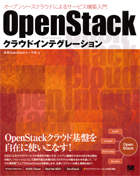
\includegraphics[scale=0.1]{OpenStack_Integration_book.png}~
\includegraphics[scale=0.1]{InfraCI_book.png}
      \begin{itemize}
      \item \href{https://www.amazon.co.jp/dp/4798139785/}{\scriptsize{OpenStack
        Cloud Integration (OpenStack クラウドインテグレーション)}}
      \item \href{https://www.amazon.co.jp/dp/4798155128/}{\scriptsize{Infra CI
        Pragmatic Guide - Ansible/GitLab (インフラ CI 実践ガイド)}} (as a reviewer)
      \end{itemize}
    \item Hobby
      \begin{itemize}
      \item Bike, Diet, Clouds, etc. \\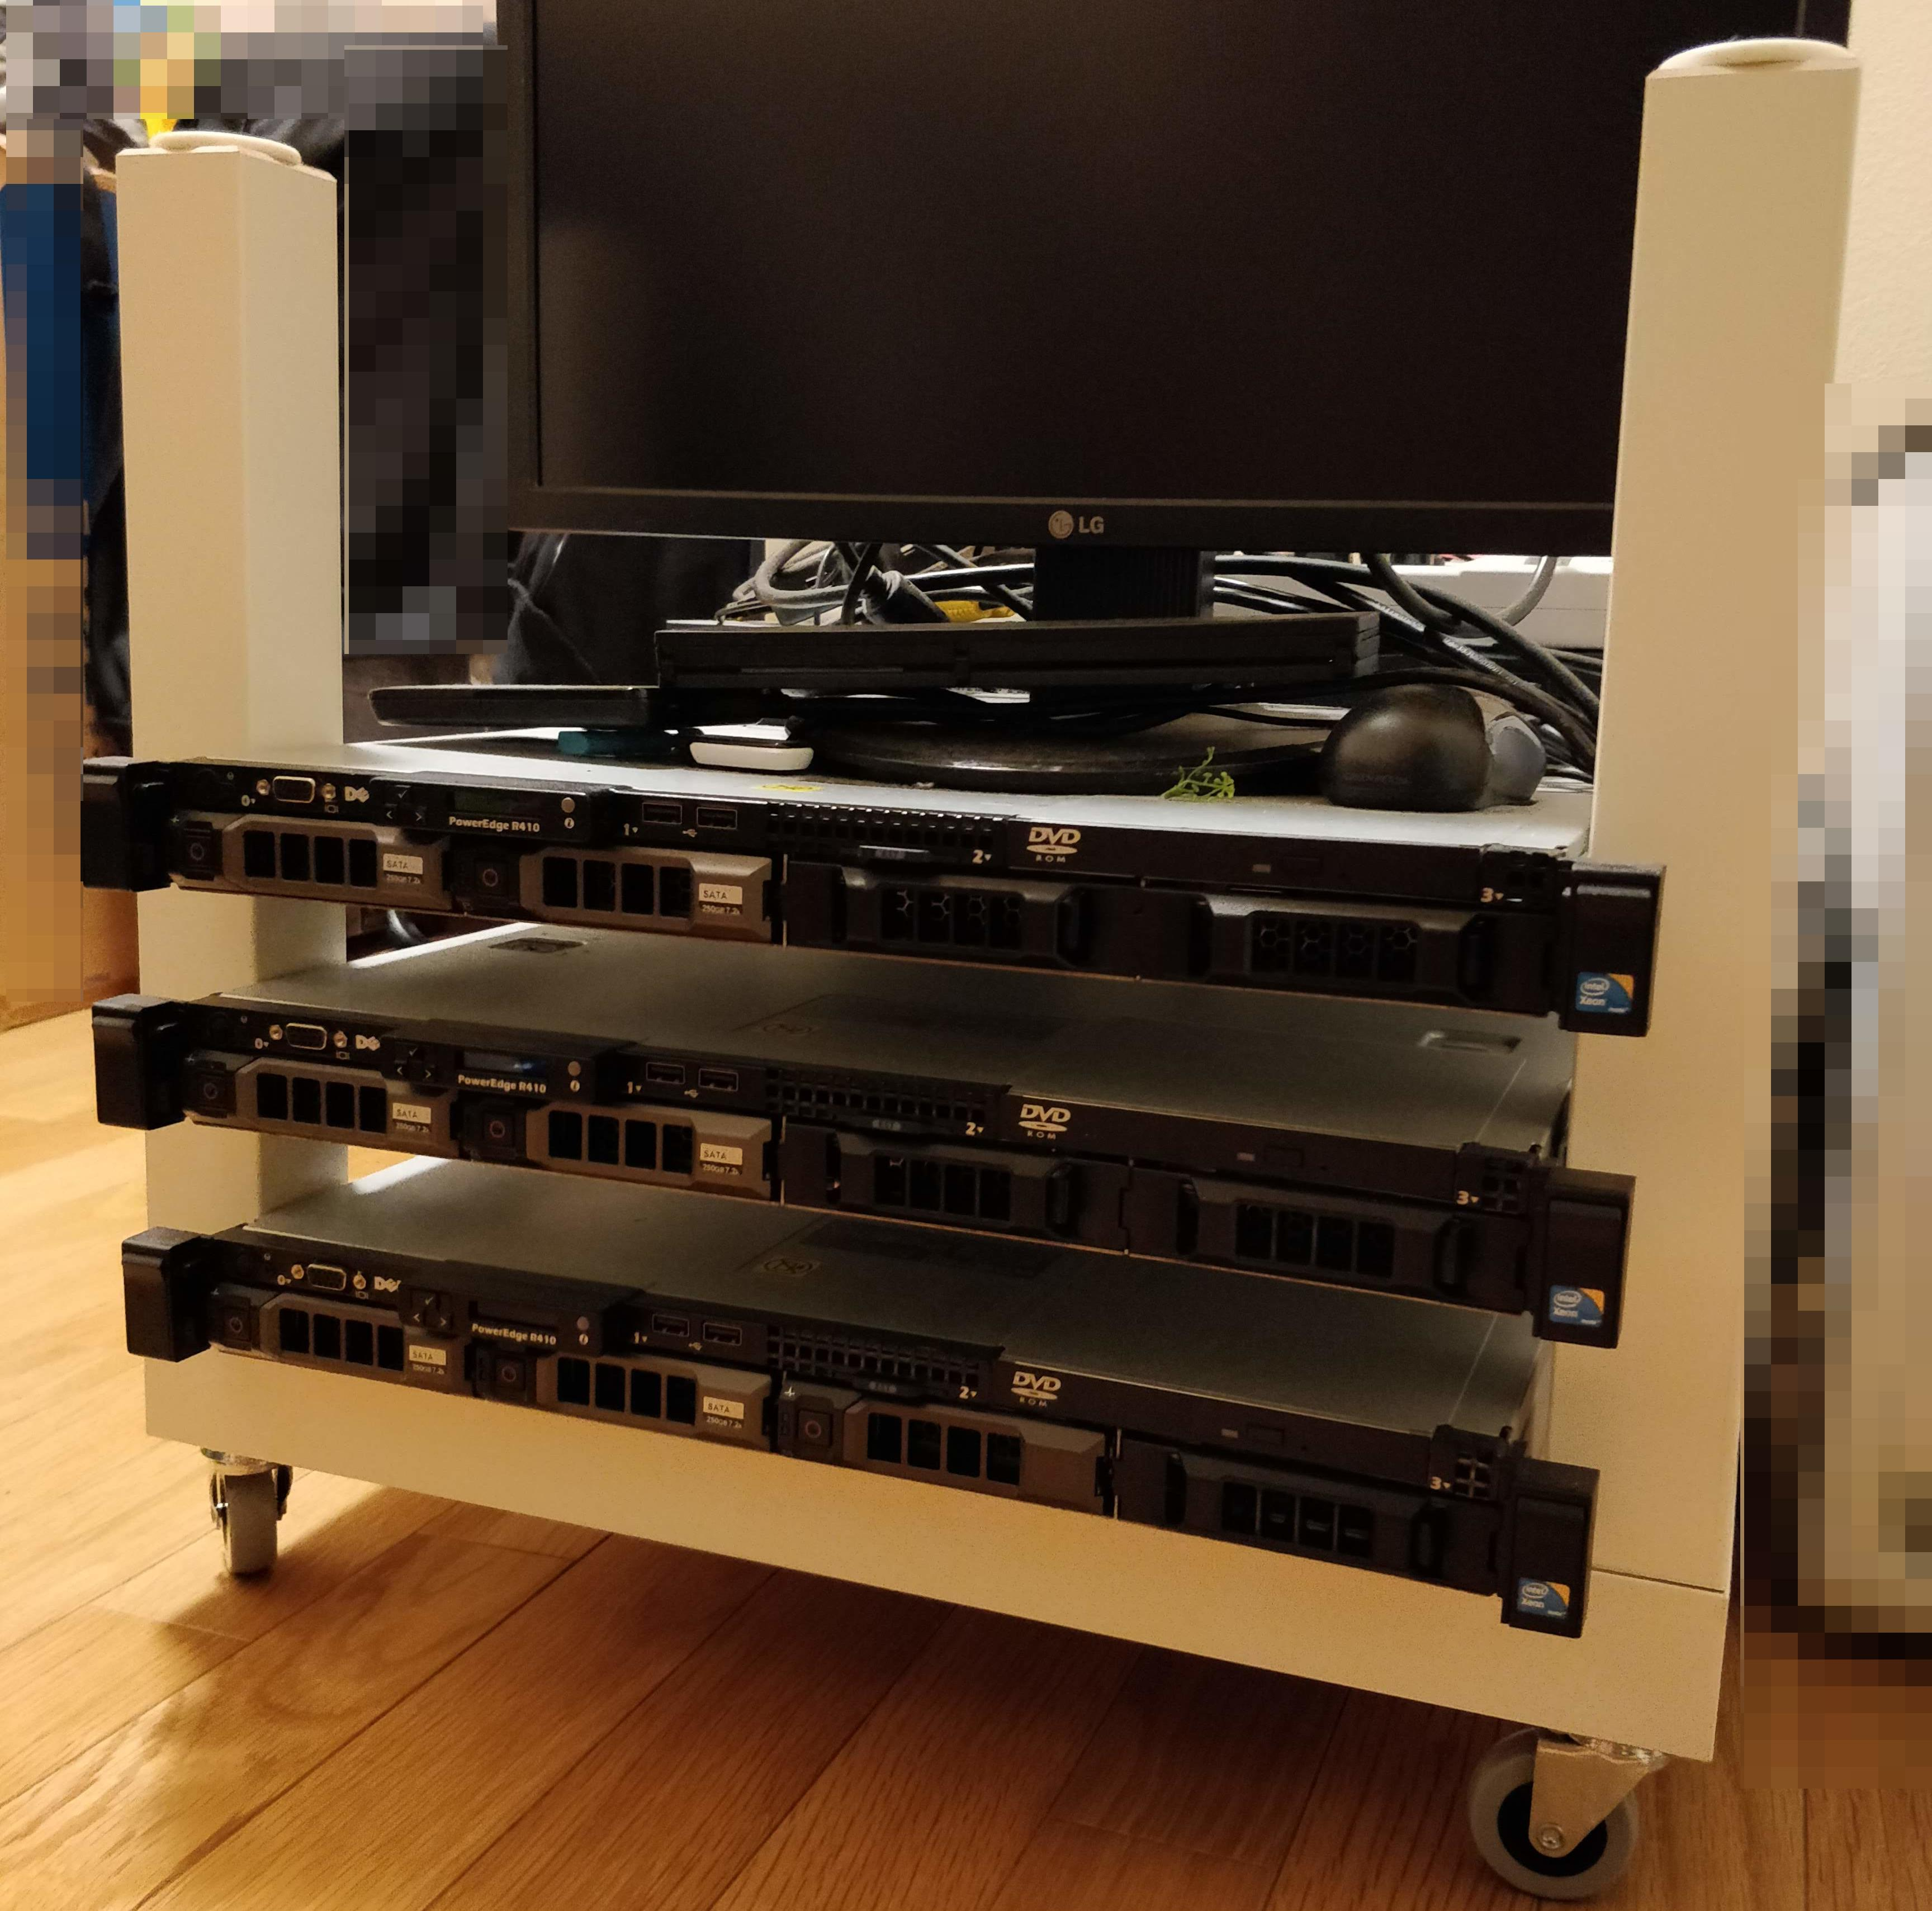
\includegraphics[scale=0.05]{server_front.jpg}
      \end{itemize}
  \end{itemize}
\end{frame}

\section{Goal of today}
\begin{frame}
  \frametitle{今日のゴール}
  \begin{itemize}
    \item OpenStack/OSS 開発手法・使われているツールをざっくり理解する
    \item 開発していく上でのハマりどころを理解する
  \end{itemize}
\end{frame}

\section{What is the ``OpenStack''?}
\begin{frame}
  \frametitle{``OpenStack'' とは?}
  \begin{itemize}
    \item Open Source Cloud Operation System: Apache License Version 2.0
    \item Written in Python
    \item There are a lot of `OpenStack' projects: \href{http://governance.openstack.org/reference/projects/index.html}{63 projects(2018-10-23)}
    \item Released every 6 month: Latest version is called `Queens'
    \item Users: \scriptsize{AT\&T, AA, BBVA, Bloomberg, CERN,
      China Mobile, Gap, VEXXHOST,
      Volkswagen, WALMART, etc.. \url{https://www.openstack.org/user-stories/}}
  \end{itemize}
  \begin{center}
    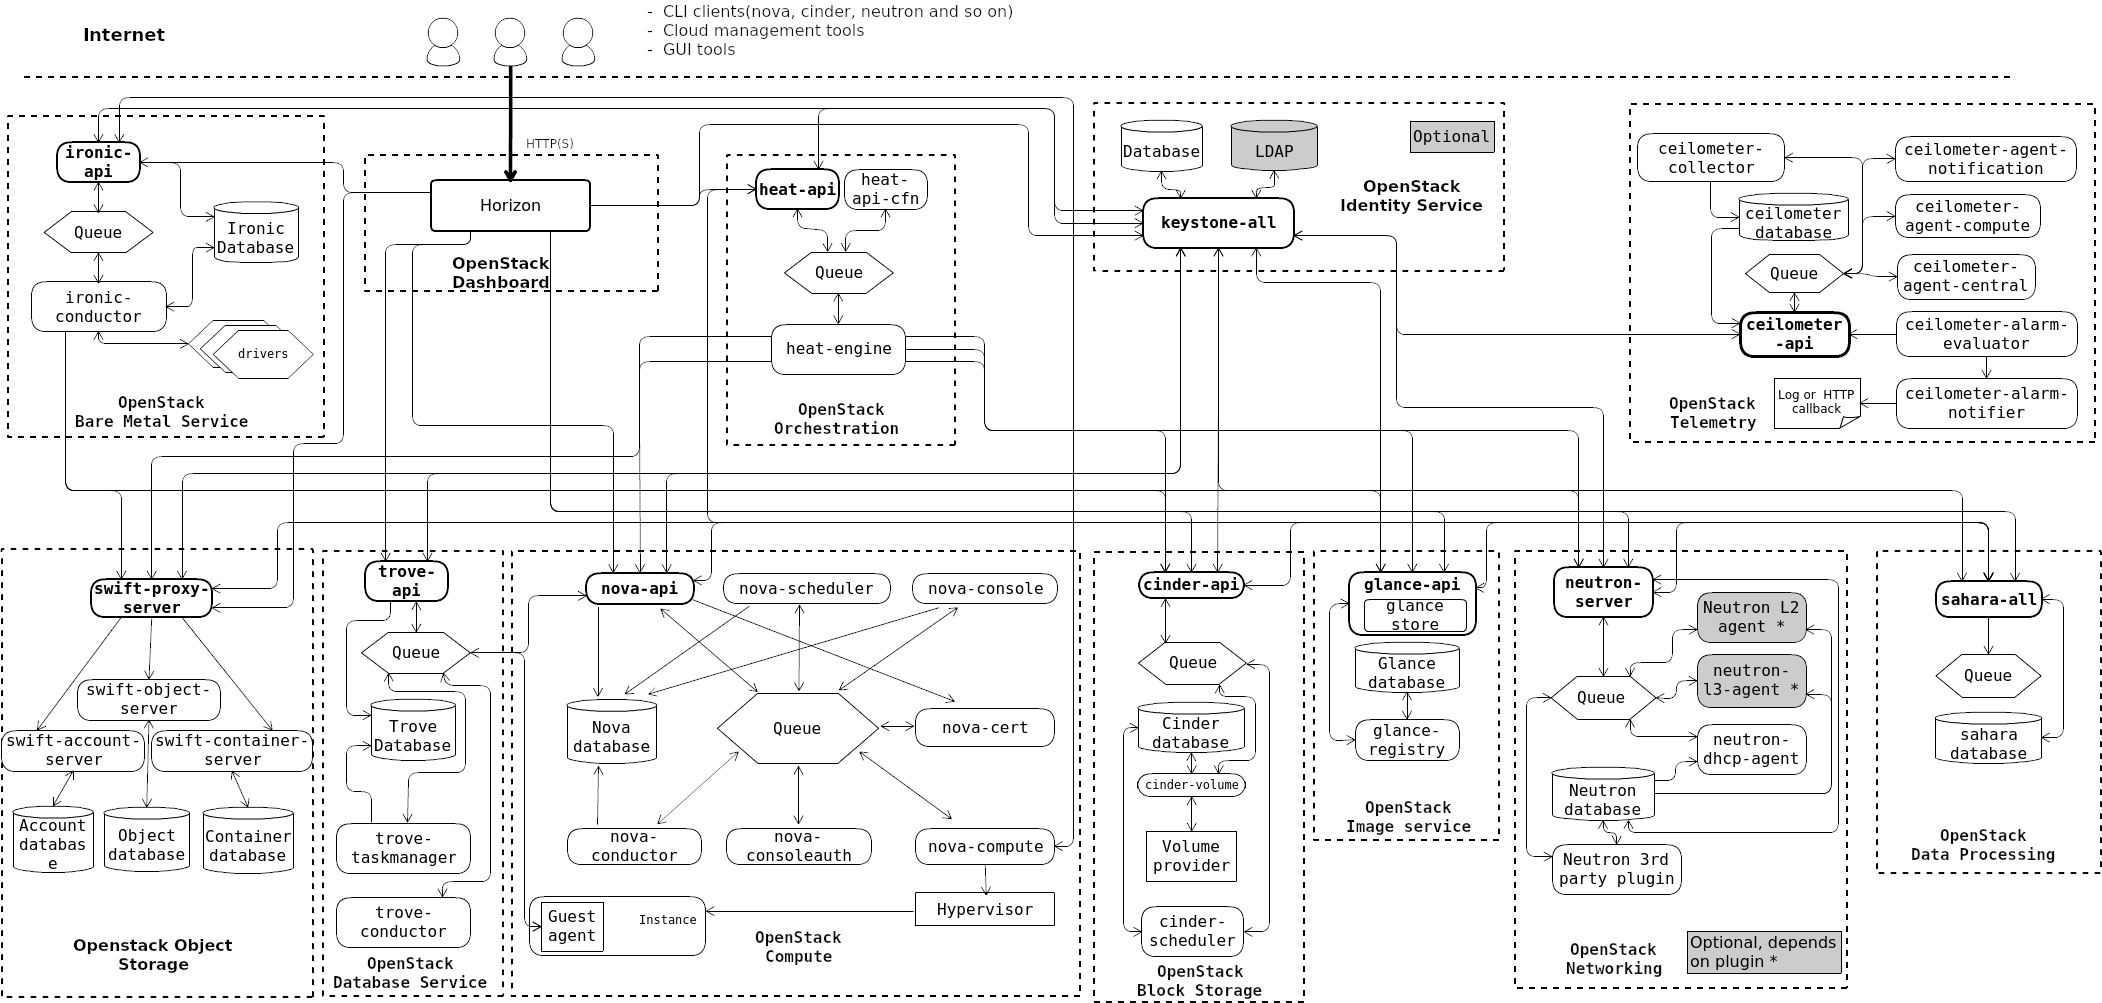
\includegraphics[width=0.7\textwidth]{openstack-arch-kilo-logical-v1.png}
  \end{center}
\end{frame}

\section{Workflow of OpenStack development}
\begin{frame}
  \frametitle{OpenStack の開発ワークフロー}
  \begin{enumerate}
    \item StoryBoard へ ストーリー登録&議論 (Option)
    \item パッチ作成、Gerrit でパッチ登録
    \item Zuul にて CI 自動実行
    \item Gerrit 上で レビュー
    \item CI再度実行後、メインリポジトリへマージ
  \end{enumerate}
\end{frame}

\section{Conclusion}
\begin{frame}
  \frametitle{Conclusion}
  \begin{itemize}
    \item OpenStack 開発では、Gerrit, StoryBoard, Zuul 等様々なOSSが使われていて、皆さんの開発でも利用することができます。
    \item 英語重要
    \item OSS 開発は楽しい!皆さん参加しましょう!
  \end{itemize}
\end{frame}

\end{document}
